
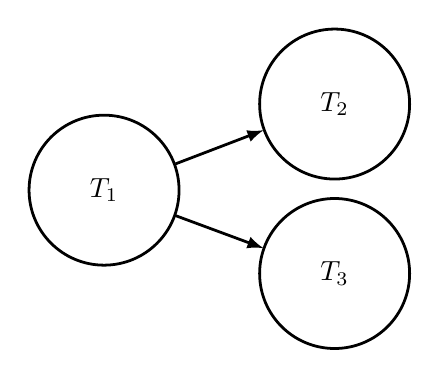
\begin{tikzpicture}[>=latex,line join=bevel,]
  \pgfsetlinewidth{1bp}
%%
\pgfsetcolor{black}
  % Edge: T_1 -> T_2
  \draw [->] (52.743bp,66.469bp) .. controls (59.73bp,69.144bp) and (67.459bp,72.102bp)  .. (84.409bp,78.589bp);
  % Edge: T_1 -> T_3
  \draw [->] (52.743bp,47.836bp) .. controls (59.73bp,45.248bp) and (67.459bp,42.386bp)  .. (84.409bp,36.108bp);
  % Node: T_2
\begin{scope}
  \definecolor{strokecol}{rgb}{0.0,0.0,0.0};
  \pgfsetstrokecolor{strokecol}
  \draw (110bp,88bp) ellipse (27bp and 27bp);
  \draw (110bp,88bp) node {$T_2$};
\end{scope}
  % Node: T_3
\begin{scope}
  \definecolor{strokecol}{rgb}{0.0,0.0,0.0};
  \pgfsetstrokecolor{strokecol}
  \draw (110bp,27bp) ellipse (27bp and 27bp);
  \draw (110bp,27bp) node {$T_3$};
\end{scope}
  % Node: T_1
\begin{scope}
  \definecolor{strokecol}{rgb}{0.0,0.0,0.0};
  \pgfsetstrokecolor{strokecol}
  \draw (27bp,57bp) ellipse (27bp and 27bp);
  \draw (27bp,57bp) node {$T_1$};
\end{scope}
%
\end{tikzpicture}

